\section{Automi a Pila}
Come preannunciato in [[Linguaggi Context-free]], gli automi a pila sono un metodo per definire alcuni \textit{linguaggi non regolari}.
Gli automi a pila (\textit{pushdown automata}, o \textit{PDA}) sono degli automi a cui viene affiancata una memoria detta 
\g{stack} (pila), e sono \g{computazionalmente equivalenti alle grammatiche context-free}. 
Un PDA può scrivere simboli nella pila e rileggerli in seguito. Scrivere un simbolo comporta "\textit{spingere giù}" i simboli della pila.
In qualsiasi momento il simbolo nella cima può essere letto e rimosso, esattamente come si comporta una memoria di tipo \textit{stack},
e dunque \g{LIFO} (last in first out).
Un automa a pila è composto da: 
\begin{itemize}
	\item \g{Input}: stringa di caratteri dell'alfabeto
	\item \g{Memoria}: stati + pila
	\item \g{Funzioni di transizione}: dato lo stato corrente, un simbolo di input ed il \textit{simbolo in cima alla pila},
		stabilisce quali possono essere gli stati successivi e i \textit{simboli da scrivere sulla pila}
\end{itemize}
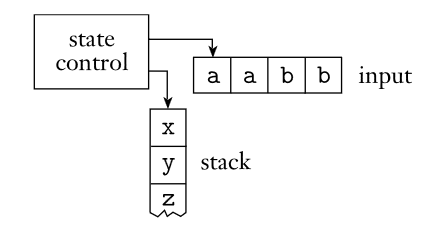
\includegraphics[scale=0.5]{img/schema_PDA.png}

Le operazioni di scrittura sono 
\begin{itemize}
	\item \g{push}: inserimento di un simbolo nella pila
	\item \g{pop}: lettura e rimozione di un simbolo dalla pila
\end{itemize}
Questo permette agli automi a pila di avere \textit{memoria infinita} \g{MA} \textit{con accesso limitato}.
Esempio: $\{0^n1^n | n \geq 0\}$

Un PDA usa la pila per contare 0 e 1:
\begin{itemize}
	\item legge i simboli in input, e *scrive* ogni 0 letto sulla pila
	\item non appena vede gli 1, *cancella* uno 0 dalla pila per ogni 1 letto
	\item se l’input termina esattamente quando la pila si svuota, **accetta**
	\item se ci sono ancora 0 nella pila al termine dell’input, *rifiuta*
	\item se la pila si svuota prima della fine dell’input, *rifiuta*
	\item se qualche 0 compare nell’input dopo gli 1, *rifiuta*
\end{itemize}


\begin{center}
	\Large\g{Attenzione}
\end{center}

Gli automi a pila possono essere \g{non deterministici}.
Automi a pila deterministici e non deterministici \textit{non} sono computazionalmente equivalenti, diversamente da quanto avviene tra DFA e NFA. 

\subsection{Definizione di PDA}
La definizione è simile a quella di un automa finito, tranne che per la pila. 
Tale pila *non utilizza necessariamente lo stesso linguaggio della stringa in input*
Per tanto un automa a pila è una sestupla $P=(Q,\Sigma,\Gamma,\delta, q_0, F)$:
\begin{itemize}
	\item $Q$ è l'insieme finito di \textit{stati}
	\item $\Sigma$ è l'alfabeto di \textit{input}
	\item $\Gamma$ è l'alfabeto della \textit{pila}
	\item $\delta:Q\times\Sigma_\varepsilon \times\Gamma_\varepsilon\mapsto 2^{Q\times\Gamma_\varepsilon}$ è la funzione di transizione
	\item $q_0\in Q$ è lo \textit{stato iniziale}
	\item $F\subseteq Q$ è l'insieme di \textit{stati accettanti} (dove $\Sigma_\varepsilon = \Sigma\cup\{\varepsilon\}$ e $\Gamma_\varepsilon = \Gamma\cup \{\varepsilon\}$)
\end{itemize}
\paragraph{Esempio}
\g{PDA per} $\{0^n1^n\mid n\geq 0\}$:\\
\begin{itemize}
\item $P = (\{q_0, q_1, q_2, q_3\}, \{0,1\}, \{0,\$\}, \delta,q_0,\{q_0,q_3\})$ 
\item con $\delta$ descritta dalla tabella:
	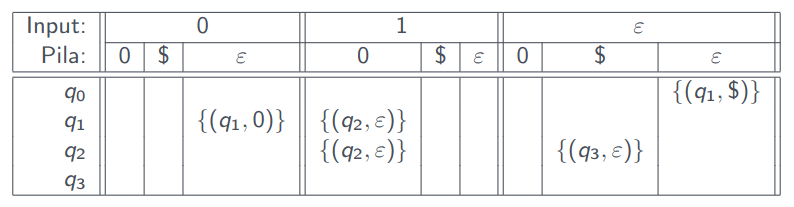
\includegraphics[scale=0.5]{img/tabella_delta.png}
	o dalla transizione
	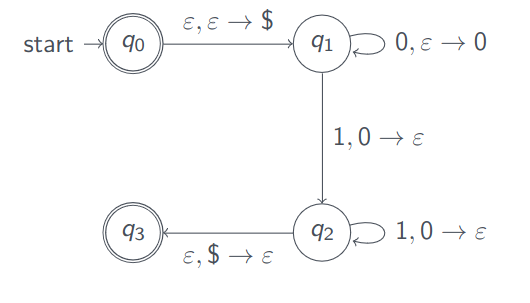
\includegraphics[scale=0.5]{img/transizione_delta.png}
\end{itemize}

\subsection{Computazione e linguaggi di un PDA}
Data una parola $w$, un PDA accetta la parola se:
\begin{itemize}
	\item possiamo scrivere $w = w_1w_2 \dots w_m$ dove $w_i \in \Sigma\cup \{\varepsilon\}$ 
	\item esistono una sequenza di stati $r_0, r_1,\dots, r_m \in Q$ e
	\item *una sequenza di stringhe* $s_0, s_1, s_2,\dots, s_m \in \Gamma^*$ 
\end{itemize}
\begin{center}
	tali che
\end{center}
\begin{enumerate}
	\item $r_0 = q_0$ e $s_0 = \varepsilon$ (inizia dallo stato iniziale e pila vuota)
	\item per ogni $i = 0, \dots, m - 1, (r_i+1, b) \in \delta(r_i , w_{i+1}, a)$ con $s_i = at$
		e $s_{i+1} = bt$ per qualche $a, b\in \Gamma_\varepsilon$ e $t\in\Gamma^*$ (l'automa rispetta la funzione
		di transizione)
	\item $r_m\in F$ (la computazione *termina in uno stato finale*)
\end{enumerate} 

\subsection{Accettazione per pila vuota}
La nostra definizione di PDA accetta le parole \textit{per stato finale}.
L'accettazione per pila vuota costituisce un altro un altro modo per definire la \textit{condizione di accettazione}:
Un PDA accetta la parola $w$ per pila vuota se esiste una computazione che
\begin{itemize}
	\item consuma tutto l’input
	\item termina con la pila vuota $(s_m = \varepsilon)$ 
\end{itemize}
\g{Equivalenza}\
\begin{theorem}
	Per ogni linguaggio accettato da un PDA per stato finale esiste un
	PDA che accetta per pila vuota, e viceversa
\end{theorem}

\begin{theorem}[Equivalenza con le grammatiche context-free]
	Un linguaggio è context-free se e solo se esiste un PDA che lo riconosce.
\end{theorem}
Sappiamo che un linguaggio è context-free se esiste una CFG che lo genera 
Mostreremo come trasformare la grammatica in un PDA e, viceversa, come trasformare un PDA in una grammatica. 

\begin{lemma}
	Se un linguaggio è context-free, allora esiste un PDA che lo riconosce
\end{lemma}
Per fare convertire una CFG in PDA è importante tenere a mente che ogni passo di derivazione produce una **stringa intermedia** contenente variabili e terminali.
Data una stringa $w$ il PDA dev'essere progettato in modo da stabilire se una serie di sostituzioni effettuate secondo le regole della CFG possa condurre dalla variabile iniziale a $w$.
Per fare questo è fondamentale sfruttare il **non determinismo** del PDA per poter effettuare le sostituzioni che portano a $w$. 
Il PDA inizia scrivendo la variabile iniziale sulla pila. 

\g{Idea}:
\begin{itemize}
	\item Se $L$ è context-free, allora esiste una CFG $G$ che lo genera
	\item Mostriamo come trasformare $G$ in un PDA equivalente $P$
	\item $P$ è fatto in modo da *simulare* i *passi di derivazione* di $G$
	\item $P$ accetta $w$ se esiste una derivazione di $w$ in $G$
\end{itemize}

\subsubsection{Rappresentare le stringhe intermedie}
\begin{itemize}
	\item La **pila** memorizza le stringhe intermedie
	\item $P$ trova le variabili nella stringa intermedia e fa le sostituzioni
  	seguendo le regole di $G$ 
	\item **Idea**: metto nella pila solo **i simboli dalla prima variabile in poi**
		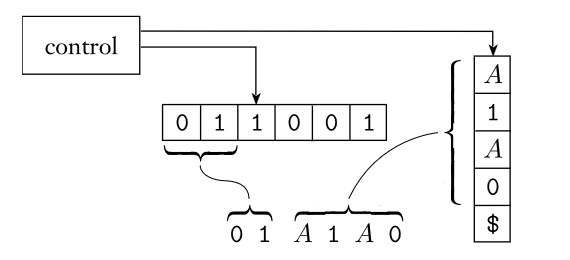
\includegraphics[scale=0.5]{img/stringhe_intermedie.png}
	\item Ogni derivazione è una sequenza di **stringhe intermedie**
\end{itemize}

$S\rightarrow 0S1\mid\varepsilon$ 
$S\Rightarrow 0S1\Rightarrow 00S11\Rightarrow 0011$
L'automa partirà dalla variabile iniziale, poi supponiamo che l'automa si trovi in $00S11$ 
Grazie alle transizioni elaborate avremo la pila 

0
0
S  In questo caso l'automa trova una variabile e applica una regola $(0S1\mid\varepsilon)$
1
1
\$  Ad indicare la fine della pila 

\subsection{Definizione informale del PDA}
\begin{enumerate}
	\item Inserisci il simbolo marcatore $\$$ e la variabile iniziale $S$  sulla pila
	\item  Ripeti i seguenti passi:
		\begin{enumerate}
			\item Se la cima della pila è la variabile $A$: scegli una regola $A\rightarrow u$ e 
				scrivi $u$ sulla pila (qui si sfrutta il non determinismo )
			\item Se la cima della pila è un terminale $a$: leggi il prossimo simbolo
				di input.
				\begin{itemize}
					\item se sono uguali, procedi
					\item se sono diversi, rifiuta
				\end{itemize}
		\end{enumerate}
	\item Se la cima della pila è $\$$: vai nello stato accettante
\end{enumerate}

\subsection{Notazione compatta}
Supponiamo che il PDA vada da $q$ z $r$ quando legge $a$ e fa il pop di $s$ 
... inserendo la **stringa** di tre caratteri $u=xyz$ sulla pila, per farlo sono necessarie 3 transizioni come nell'immagine 
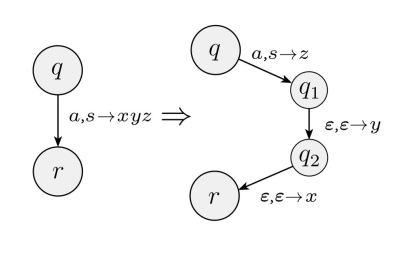
\includegraphics[scale=0.5]{img/notazione_compatta.png}

Per implementare il push multiplo dobbiamo **aggiungere stati ausiliari**  

\subsection{Dimostrazione}
Data $G=(V,\Sigma, R, S)$ definiamo $P=(Q,\Sigma,\Gamma,q_{start},F)$ 
\begin{itemize}
	\item $Q=\{q_{start}, q_{loop}, q_{end}\}$ 
	\item $\Gamma = \Sigma \cup V \cup \{\$\}$ 
	\item $F=\{q_{end}\}$ 
	\item funzione di transizione
\end{itemize}
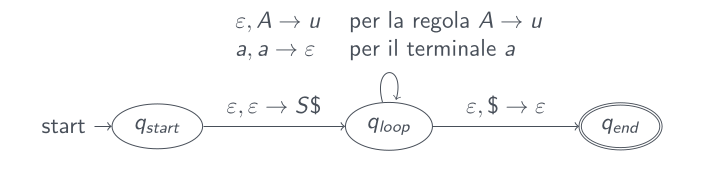
\includegraphics[scale=0.5]{img/dimostrazione_pda.png}

\subsection{Da PDA a grammatica Context-Free}
Abbiamo un PDA $P$ che riconosce il linguaggio 
Mostriamo come trasformare $P$ in una CFG equivalente $G$ 
\begin{itemize}
	\item Una stringa $w$ accetta da $P$ se fa andare $P$ dallo stato iniziale a quello finale
	\item Progetteremo una grammatica che **fa un po' di più** 
		\begin{itemize}
			\item Una variabile $A_{pq}$ per ogni coppia di stati $p,q$ di $P$ 
			\item $A_{pq}$ genera tutte le stringhe che portano **da** $p$ **con pila vuota** a $q$ **con pila vuota**
		\end{itemize}
\end{itemize}
Come prima cosa, semplifichiamo $P$ in modo che rispetti tre condizioni:
\begin{enumerate}
	\item ha un unico stato accettante $q_f$ 
	\item svuotiamo la pila prima di accettare
	\item  Ogni transizione **inserisce un unico simbolo sulla pila (push)** oppure **elimina un simbolo dalla pila (pop)**, ma non fa entrambe le cose contemporaneamente. 
\end{enumerate}

\paragraph{Andare da $P$ a $q(1)$}
Per andare da $p$ con pila vuota a $q$ con pila vuota:
\begin{itemize}
	\item la prima mossa deve essere necessariamente un push 
	\item l'ultima mossa deve essere un pop
\end{itemize}
Ci sono due casi:
\begin{enumerate}
	\item Il simbolo inserito all'inizio viene eliminato alla fine:
		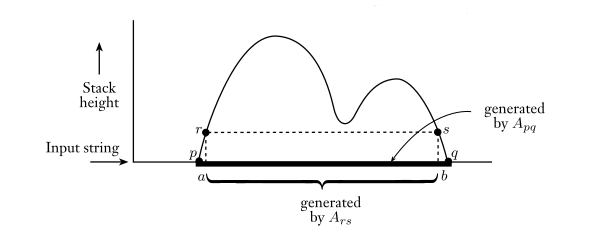
\includegraphics[scale=0.5]{img/da_p_a_q.png}
		Per ogni coppia di transizioni che effettuano il push e il pop di un determinato simbolo andremo ad aggiungere una regola:
		$A_{pq}\rightarrow aA_{rs}b$ 
	\item Oppure no, il simbolo inserito all'inizio viene rimosso prima di terminare la computazione.
		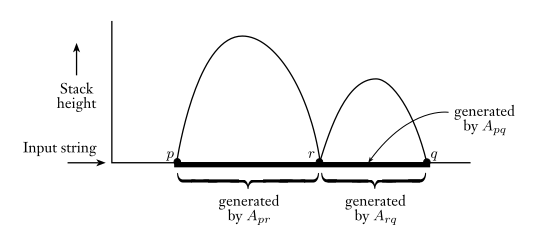
\includegraphics[scale=0.5]{img/da_p_a_q_2.png}
		in questo caso dobbiamo aggiungere la regola
		$\forall p,q,r\in Q$ 
		$A_{pq}\rightarrow A_{pr}A_{rq}$
		$A_{pq} \rightarrow\varepsilon$ per ogni $q\in Q$ 
\end{enumerate}

\paragraph{Le regole di $G$}
Formalmente 
\begin{itemize}
	\item sia $P=(Q,\Sigma,\Gamma, \delta, q_0,\{q_r\})$ 
	\item costruiamo $G=(V\Sigma, R, A_{q0}, q_r)$ tale che 
		\begin{itemize}
			\item $V =\{A_{pq}, p, q\in Q \}$
			\item Per ogni $p,q,r,s,\in Q$, $u\in\Gamma$ e $a,b\in\Sigma$, se $\delta(p,a,\varepsilon)$ contiene $(r,u)$ e $\delta(s,b,u)$ contiene $(q,\varepsilon$ ), aggiungi la regola $A_{pq}\rightarrow aA_{rs}b$ 
			\item Per ogni $p,q,r,\in Q$, aggiungi la regola $A_{pq}\rightarrow A_{pr}A_{rq}$ 
			\item Per ogni $p\in Q$, aggiungi la regola $A_{pp}\rightarrow \varepsilon$ 
		\end{itemize}
\end{itemize}

\paragraph{Due dimostrazioni induttive}
\paragraph{Lemma}
Se $A_{pq}$ genera la stringa $x$, allora $x$ può portare $P$ da $p$ con pila vuota a $q$ con pila vuota
\paragraph{Lemma}
Se la stringa $x$ può portare $P$ da $p$ con pila vuota a $q$ con pila vuota, allora $A_{pq}$ genera $x$. 

\begin{theorem}
	Un linguaggio è context-free se e solo se esiste un PDA che lo rionosce 
\end{theorem}
\begin{itemize}
	\item Sappiamo che un linguaggio è context-free se esiste una CFG che lo genera
	\item Abbiamo mostrato come trasformare una CFG in un PDA
	\item E viceversa, come trasformare un PDA in grammatica
\end{itemize}



